
\documentclass[10pt,conference]{IEEEtran}

\usepackage{cite}
\usepackage{amsmath,amssymb,amsfonts}
\usepackage{amsthm}
\usepackage{algorithm}
\usepackage{algpseudocode}
\usepackage{booktabs}
\usepackage{array}
\usepackage{url}
\Urlmuskip=0mu plus 1mu\relax
\def\UrlBreaks{\do\/\do-\do\_\do\.}
\usepackage{tikz}
\usetikzlibrary{positioning,arrows.meta,calc,fit,shapes.geometric}
\usepackage{pgfplots}
\pgfplotsset{compat=1.17}

\newtheorem{definition}{Definition}
\newtheorem{theorem}{Theorem}
\newtheorem{lemma}{Lemma}
\newtheorem{invariant}{Invariant}

\newcommand{\bep}{BEP-IR}
\newcommand{\unknown}{\mathsf{unknown}}
\newcommand{\allow}{\mathsf{allow}}
\newcommand{\block}{\mathsf{block}}
\newcommand{\monitor}{\mathsf{monitor}}
\newcommand{\clear}{\mathsf{clear}}

\begin{document}

\title{BEPGuard: Proof-Carrying Evidence for Policy Intent Drift in Browser-Enforced Security Policy Engineering}
\author{\IEEEauthorblockN{Anonymous Author(s)}}
\maketitle

\begin{abstract}
Browser-enforced security policies are maintained as advice, framework defaults, middleware options, migration notes, and CI checks, but browsers enforce them through delivery state, request context, cache state, and cross-policy composition. This paper studies \emph{policy intent drift}: a synchronic inconsistency, measured at one evaluation point, among an explicit developer-facing claim, a generated policy surface, and the browser-effective judgment. We introduce \bep, an executable representation for those objects, and BEP-Deep, a repair-paired semantic workload derived from 45 public claims and 35 encoded rules across CSP, CORS, HSTS, COEP/CORP/CORS, COOP/COEP, and Permissions-Policy. BEP-Deep contains 972 deterministic fixtures: 418 expected conflicts and 554 negative controls, including one paired repair control for every positive witness. The generator detects all expected conflicts and keeps all controls clean, but the important result is not the all-pass count by itself. A second decision-table oracle, a label-free declarative oracle, finite-state contracts, obligation-level mutants, proof-carrying certificates, identifier-blind replay, causal activation, repair-delta replay, benchmark-disjointness checks, and BEP-Max adversarial validation all test whether the findings survive without fixture-name or scanner-score shortcuts. Precomputed and archived public-package comparator outputs provide contrastive evidence about scanner/task mismatch; the labels remain source-grounded semantic obligations. The result is a semantic regression object for policy engineering: intent, generated policy, effective enforcement, witness, certificate, and counterfactual repair are checked together, so a maintainer can see which policy relation failed and what local repair must preserve.
\end{abstract}

\begin{IEEEkeywords}
software engineering, software security, web security, configuration analysis, formal semantics, empirical software engineering
\end{IEEEkeywords}

\section{Introduction}

Modern web applications delegate substantial parts of their browser-side security posture to browser-enforced policies. Content Security Policy (CSP) constrains script and resource loading; Cross-Origin Resource Sharing (CORS) decides whether responses can be shared with credentialed cross-origin callers; HTTP Strict Transport Security (HSTS) changes a user agent's future transport behavior; Cross-Origin Embedder Policy (COEP), Cross-Origin Resource Policy (CORP), and Cross-Origin Opener Policy (COOP) shape embedding and isolation; and Permissions-Policy disables selected browser features \cite{w3c_csp3_2026,whatwg_fetch_2026,rfc6797_hsts,w3c_corp_2026,whatwg_html_coop_2026,w3c_permissions_policy_2026}. These mechanisms are security policies, but in practice they are also software-engineering maintenance objects: they are generated by frameworks, configured through middleware APIs, copied from documentation, revised during upgrades, and checked in CI.

The engineering problem is that the unit developers manipulate is rarely the unit the browser enforces. A documentation claim may say that a policy blocks third-party scripts; the application may emit only a report-only CSP header. A framework guide may recommend nonce-based CSP; the rendering architecture may be static, cached, or build-time generated, preventing per-request nonces. A CORS middleware may reflect request origins; the security consequence depends on credentials mode and response headers. An HSTS header may be present; it may still be ignored when delivered over insecure transport, or it may clear stored state through a zero max-age directive. A page may set COEP; embedding still depends on the requested resource's CORS/CORP surface. Existing developer tools and scanners are useful, but they often evaluate one header, one syntax, or one grade rather than the relation among explicit intent, generated policy, and browser-effective semantics \cite{google_csp_evaluator_2026,mdn_http_observatory_2026}.

We call this relation \emph{policy intent drift}. The term names a source-grounded inconsistency at one evaluation point, rather than a historical change in browser engines: a public policy claim entails an expected browser action, a generated policy surface is associated with that claim, and the modeled browser-effective judgment contradicts the expected action in a covered context. The contribution is therefore not another security-header checklist. It is a method for turning policy-engineering claims into executable semantic obligations and for producing minimal witnesses when those obligations fail.

The difficulty is that browser-enforced policies are heterogeneous. CSP uses delivery disposition and directive fallback; CORS is a request/response protocol with credentials and preflights; HSTS is stateful; COEP/CORP/CORS interact through request mode and embedding; Permissions-Policy uses allowlists. Prior work has studied CSP deployment and whitelist weaknesses \cite{weichselbaum_csp_dead_2016,calzavara_content_security_problems_2016,calzavara_csp_semantics_2018,roth_complex_csp_2020}, CORS deployment pitfalls \cite{chen_cors_2018}, cross-policy inconsistency at web scale \cite{calzavara_site_policy_2021}, and browser implementation differences \cite{wi_diffcsp_2023}. Those results motivate a different SE question: how can a maintainer or researcher evaluate whether policy intent, framework generation, and browser semantics agree, without relying on live scanning, private data, or a scanner-specific grading rubric?

This paper makes four contributions. The novelty is the SE evaluation discipline that makes browser-policy semantics reviewable across policy families: an admitted cross-family representation, proof-carrying witnesses with counterfactual repairs, and independent release gates that can falsify overfitted evidence.
First, we define \bep, an intermediate representation that links explicit public policy claims, generated policy surfaces, contexts, and browser-effective judgments across CSP, CORS, HSTS, COEP/CORP/CORS, COOP/COEP, and Permissions-Policy mechanisms.
Second, we define policy intent drift and minimal semantic conflict witnesses. A witness is a small policy/context object that explains a contradiction; it is designed for debugging and reproducibility rather than for ranking websites.
Third, we provide algorithms and proof obligations for normalization, effective judgment evaluation, witness generation, minimization, repair validation, and proof-carrying witness certification.
Fourth, we evaluate the method on a locked deterministic corpus: 45 explicit claims, 35 semantic rules, 972 BEP-Deep fixtures, 418 expected-positive conflicts, and 554 negative controls. The evaluation reports coverage, minimization, repair synthesis, certificates, ablations, adversarial validation, external comparator execution, finite theory checking, mutation adequacy, oracle independence, anti-overfit replay, traceability, and release-reproducibility checks summarized in Table~\ref{tab:strata}.

The paper's central thesis is that browser-policy maintenance requires a semantic evaluation object rather than a header checklist: each claim must be checked against the generated surface and the browser-effective judgment that surface induces.

\section{Motivating Evidence and Research Questions}

\paragraph{Three surfaces, one engineering obligation}

Figure~\ref{fig:drift-model} shows the paper's central object. Browser-policy engineering spans three surfaces. The \emph{intent surface} consists of explicit public claims: normative specification text, browser documentation, framework documentation, migration guides, and developer-facing examples. The \emph{generation surface} is the header or policy object emitted by framework APIs, middleware defaults, application code, or deployment layers. The \emph{effective surface} is the browser judgment after delivery mode, fallback/default rules, request context, browser state, and composition rules are applied.

\begin{figure}[t]
\centering
\definecolor{cmbInk}{RGB}{27,31,36}
\definecolor{cmbBlue}{RGB}{43,82,125}
\definecolor{cmbTeal}{RGB}{43,125,116}
\definecolor{cmbGold}{RGB}{158,116,49}
\definecolor{cmbRose}{RGB}{151,75,82}
\definecolor{cmbMist}{RGB}{239,245,249}
\definecolor{cmbMint}{RGB}{237,247,244}
\definecolor{cmbWarm}{RGB}{248,244,235}
\definecolor{cmbRule}{RGB}{196,202,205}
\begin{tikzpicture}[
  panel/.style={draw=#1, fill=#1!7, rounded corners=2.6pt, line width=.58pt,
    align=center, minimum height=.86cm, minimum width=2.18cm,
    inner xsep=2.4pt, inner ysep=2.0pt,
    font=\rmfamily\fontsize{7.2}{7.8}\selectfont, text=cmbInk,
    text height=1.35ex, text depth=.28ex},
  tag/.style={font=\rmfamily\fontsize{6.55}{7.1}\selectfont, text=black!58,
    align=center, inner sep=.45pt, text height=1.22ex, text depth=.24ex},
  flow/.style={-{Latex[length=1.8mm]}, line width=.72pt, draw=black!48,
    line cap=round, line join=round},
  gate/.style={draw=cmbGold, fill=cmbWarm, rounded corners=2.2pt, line width=.55pt,
    align=center, minimum height=.78cm, minimum width=3.18cm,
    inner xsep=2.2pt, inner ysep=1.8pt,
    font=\rmfamily\fontsize{7.0}{7.7}\selectfont, text=cmbInk,
    text height=1.32ex, text depth=.28ex}
]
\node[panel=cmbBlue] (intent) {Explicit public\\intent claim};
\node[panel=cmbTeal, right=.52cm of intent] (surface) {Generated policy\\surface};
\node[panel=cmbBlue, right=.52cm of surface] (judgment) {Browser-effective\\judgment};
\node[gate, below=.70cm of surface] (witness) {Minimal conflict witness\\plus repair-paired control};
\node[tag, below=.12cm of intent] (claimtag) {expected action};
\node[tag, below=.12cm of judgment] (judgetag) {observed action};
\draw[flow] (intent) -- node[tag, above=.03cm] {lower} (surface);
\draw[flow] (surface) -- node[tag, above=.03cm] {evaluate} (judgment);
\draw[flow, draw=cmbRose] (claimtag.south) .. controls +(0,-.28) and +(-1.15,.22) .. (witness.west);
\draw[flow, draw=cmbRose] (judgetag.south) .. controls +(0,-.28) and +(1.15,.22) .. (witness.east);
\draw[line width=.62pt, draw=cmbRule] ($(witness.south west)+(0.14,-.10)$) -- ($(witness.south east)+(-0.14,-.10)$)
  node[tag, midway, below=.02cm] {accepted only inside the covered context};
\end{tikzpicture}

\caption{Policy intent drift connects three surfaces: public intent claims, generated policy surfaces, and browser-effective judgments. A semantic conflict witness is emitted only when the modeled effective judgment contradicts the explicit expected action in a covered context.}
\label{fig:drift-model}
\end{figure}

Table~\ref{tab:motivation} gives compact examples. Each row is intentionally small. The problem is not that these policies are difficult to parse; the problem is that the relevant browser effect is outside the surface checked by a one-header rule.

\begin{table*}[t]
\centering
\caption{Motivating witness families and the semantic surface they exercise.}
\label{tab:motivation}
\begin{tabular}{p{0.24\textwidth}p{0.30\textwidth}p{0.36\textwidth}}
\toprule
Intent claim & Generated surface & Browser-effective contradiction \\
\midrule
Block untrusted scripts with CSP. & Report-only CSP with a restrictive script policy. & Report-only delivery monitors violations but does not enforce blocking in the modeled request \cite{w3c_csp3_2026,mdn_csp_header_2026}. \\
Use nonce-based CSP for scripts. & Static or cached rendering path with a nonce-bearing template. & Per-request nonces are incompatible with static generation or cache reuse in the documented rendering state \cite{nextjs_csp_2026,rails_csp_api_2026}. \\
Permit a credentialed API caller. & Wildcard ACAO combined with credentials. & Credentialed CORS sharing cannot be authorized by wildcard ACAO in the encoded Fetch fragment \cite{whatwg_fetch_2026,mdn_cors_2026,mdn_acao_2026,mdn_acac_2026}. \\
Ensure HSTS protection. & HSTS max-age header delivered over HTTP. & HSTS is accepted only from secure transport; a zero max-age update clears stored HSTS state \cite{rfc6797_hsts,mdn_hsts_2026}. \\
Enable cross-origin isolation. & COOP/COEP on the document only. & Isolation also depends on embedder/resource policy and CORS/CORP compatibility for embedded resources \cite{mdn_coep_2026,mdn_corp_header_2026,mdn_coop_2026}. \\
\bottomrule
\end{tabular}
\end{table*}

\paragraph{Research questions}

The study is a deterministic source-grounded fixture experiment that evaluates whether semantic obligations can be derived, checked, minimized, repaired, and independently audited.  The motivating examples define a precise target: intent drift requires an admitted public claim and a modeled contradiction at the same evaluation snapshot, not merely a broad security smell or a temporal implementation delta.  This precision gives each finding a provenance story: an auditor can inspect which claim was admitted, which rule was used, which context was required, which smaller witness preserves the contradiction, and which paired control removes it. The locked questions are:

\textbf{RQ1: Lowering.} Can explicit public policy-intent claims be lowered into traceable \bep{} obligations without relying on private data or live scanning?

\textbf{RQ2: Witness generation.} Across the covered policy families, how many locked positive semantic conflicts are detected, and are the locked negative controls kept clean?

\textbf{RQ3: Baseline/control disagreement.} Where do declared-scope baselines and controls disagree with semantic witnesses, and what semantic features explain those disagreements?

\textbf{RQ4: Component contribution.} Which semantic components are necessary for witness generation and minimization under locked ablations, robustness checks, and scalability workloads?

\textbf{RQ5: Oracle independence and adequacy.} Do independent decision rules, finite-state checks, semantic mutants, proof-carrying witness certificates, BEP-Max integrity checks, and evidence-redundancy audits support the claim that BEP-Deep is not merely a self-confirming oracle/workload pair?

\section{Web-Native Evidence and Method}

The method is CPU-native and web-native by construction. Its inputs are public specifications, public documentation, public tool documentation, public framework documentation, and deterministic fixtures derived from those sources.  This design makes the experiment reproducible as a local semantic evaluation object rather than a live scan or service-dependent measurement.

\paragraph{Source units and admission}

A source unit is admitted only if it makes an explicit claim about browser-policy behavior or about a framework/tool surface that generates such behavior. We included normative policy sources for CSP, Fetch/CORS, HSTS, CORP, COOP, and Permissions-Policy \cite{w3c_csp3_2026,whatwg_fetch_2026,rfc6797_hsts,w3c_corp_2026,whatwg_html_coop_2026,w3c_permissions_policy_2026}; browser-facing documentation for the corresponding headers \cite{mdn_csp_header_2026,mdn_cors_2026,mdn_hsts_2026,mdn_coep_2026,mdn_permissions_policy_2026}; framework documentation for Next.js, Spring Security, Django, Helmet, Rails, ASP.NET Core CORS, and Express CORS \cite{nextjs_csp_2026,spring_security_headers_2026,django_security_middleware_2026,helmet_docs_2026,rails_csp_api_2026,aspnet_core_cors_2026,express_cors_2026}; and public tool documentation for CSP Evaluator, MDN HTTP Observatory, and Chromium hstspreload \cite{google_csp_evaluator_2026,mdn_http_observatory_2026,chromium_hstspreload_2025}.

Admission separates three evidence roles. Fixture-backed claims instantiate positive or negative obligations. Context-surface claims define framework or deployment facts used by those obligations. Baseline-scope claims define the declared task of a comparator. This role separation is important because browser-policy documents mix normative requirements, compatibility notes, examples, operational advice, and performance caveats. The method admits source material broadly, but it assigns each claim a machine-checked role before execution. A new claim-coverage audit verifies that all 45 admitted claims are either fixture-backed, context-surface evidence, or baseline-scope evidence, with zero orphan claims.

\paragraph{Coding and validation}

For each admitted claim, the method records a policy family, intent class, expected action, source span, generated policy surface, and context variables. The context captures the elements needed by the covered semantic fragments: request mode, credentials mode, origin relation, resource kind, transport scheme, HSTS state, rendering mode, and embedding relation. Validation is traceability-based: every admitted claim must link to a public source span, every claim must have an explicit coverage role, every fixture-backed claim must link to a deterministic fixture, every negative control must carry a clean-control certificate, and every emitted witness must link to an encoded rule. The resulting source-claim trace is preserved as part of the evidence object, so a reviewer can follow a reported drift from public claim to rule, fixture, witness, and repair.

The amended denominator contains 45 admitted claims, 35 semantic rules, 116 base fixtures, and 972 deterministic BEP-Deep fixtures. Of the amended fixtures, 418 are expected-positive semantic conflicts and 554 are negative controls, including 418 paired repair controls. The controls prevent evaluation only on failing cases: enforced CSP controls, authorized CORS controls, cache-partitioned CORS controls, secure-transport HSTS controls, subdomain-scoped HSTS controls, and compatible COEP/CORP controls must remain clean. The release ladder groups its 111 materialized checks into source closure, semantic adequacy, oracle independence, repair validity, anti-overfit replay, external contrast, reproducibility, anonymity, paper-surface, and release-hygiene, overclaim-boundary, compiled-PDF text, public-provenance, and repository-upload families without changing labels or denominator.

The anti-overfitting checks are deliberately executable.  The implementation is scanned for locked fixture and certificate identifiers, but the stronger guard is behavioral: every locked fixture is copied to shadow objects with fresh identifiers and semantics-preserving perturbations of header case, field order, irrelevant metadata, and context noise.  All 9,720 required shadow cases preserve the expected issue signature.  A separate BEP-Scale replay applies 48,600 deterministic representation variants.  The stricter identifier-blind replay erases fixture ids, hashes, roles, expected labels, source claims, variants, and policy-family fields in five modes and re-executes 4,860 blinded objects; all preserve the expected issue signature.  Repair-delta replay then checks all 418 positive/repair pairs, including a fully blinded repaired side, so counterfactual repairs cannot depend on metadata.  The complementary causal-activation audit starts from clean controls and verifies 546/546 targeted boundary-crossing edits, while a benchmark-disjointness audit checks 9,586 benchmark-adjacent rows for fresh identifiers and explicit canonical overlaps.  These gates make overfitting visible as a validation failure rather than a matter of trust.

The validation is analogous to a deterministic audit trail rather than open qualitative coding. Qualitative methods remain relevant for defining threat constructs and ensuring that evidence categories are not arbitrary \cite{seaman_qualitative_1999,braun_clarke_thematic_2006,runeson_case_study_2012,stol_grounded_theory_2016}. However, this study does not ask independent coders to interpret developer intent. It asks whether an explicit public claim can be linked to a rule and fixture without inference. This is why the paper reports traceability validation instead of inter-rater reliability.

\begin{table}[t]
\centering
\caption{Evidence and validation ladder for the BEP-Deep evaluation object.}
\label{tab:strata}
\begin{tabular}{lr}
\toprule
Object or validation burden & Count \\
\midrule
Public claims / encoded rules & 45 / 35 \\
BEP-Deep positives / negatives & 418 / 554 \\
Positive / negative certificates & 418 / 554 \\
Decision-table agreements & 972 / 972 \\
Directive / cross-policy checks & 6; 7 / 111 \\
Finite theorem kernel / states & 30 / 33,513 \\
SpecBench cases / rules & 4,180 / 29 \\
Declarative oracle cases & 5,152 \\
Counterfactual round-trip cases & 546 \\
Oracle-equivalence cases & 5,152 \\
Rule trace-matrix obligations & 280 \\
Issue evidence obligations & 200 \\
Shadow / blind / scale replays & 9,720 / 4,860 / 48,600 \\
Causal / stability / disjointness & 546 / 2,916 / 9,586 \\
Mutation kills & 28 + 600 \\
Evidence graph nodes / edges & 15,182 / 23,925 \\
BEP-Max cases / integrity & 4,306 / 4,306 \\
Repair / issue-coverage closure & 418; 25 / 25 \\
release validation layers & 111 / 111 \\
\bottomrule
\end{tabular}
\end{table}

Figure~\ref{fig:method-pipeline} summarizes the source-to-repair path and the validation gates that make each accepted witness falsifiable.

\begin{figure*}[t]
\centering
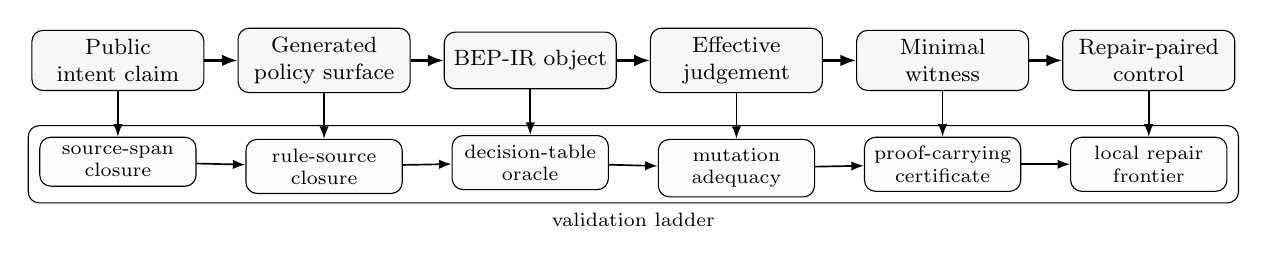
\begin{tikzpicture}[
  stage/.style={draw, rounded corners, align=center, font=\footnotesize, minimum height=0.72cm, text width=1.95cm, fill=black!3},
  gate/.style={draw, rounded corners, align=center, font=\scriptsize, minimum height=0.58cm, text width=1.75cm, fill=black!1},
  arrow/.style={-{Latex[length=2mm]}, thick},
  thinarr/.style={-{Latex[length=1.6mm]}, semithick}
]
  \node[stage] (claim) {Public\\intent claim};
  \node[stage, right=0.42cm of claim] (surface) {Generated\\policy surface};
  \node[stage, right=0.42cm of surface] (ir) {\bep\ object};
  \node[stage, right=0.42cm of ir] (judge) {Effective\\judgement};
  \node[stage, right=0.42cm of judge] (wit) {Minimal\\witness};
  \node[stage, right=0.42cm of wit] (repair) {Repair-paired\\control};

  \node[gate, below=0.58cm of claim] (source) {source-span\\closure};
  \node[gate, below=0.58cm of surface] (rules) {rule-source\\closure};
  \node[gate, below=0.58cm of ir] (dt) {decision-table\\oracle};
  \node[gate, below=0.58cm of judge] (mut) {mutation\\adequacy};
  \node[gate, below=0.58cm of wit] (cert) {proof-carrying\\certificate};
  \node[gate, below=0.58cm of repair] (frontier) {local repair\\frontier};

  \draw[arrow] (claim) -- (surface);
  \draw[arrow] (surface) -- (ir);
  \draw[arrow] (ir) -- (judge);
  \draw[arrow] (judge) -- (wit);
  \draw[arrow] (wit) -- (repair);

  \draw[thinarr] (claim) -- (source);
  \draw[thinarr] (surface) -- (rules);
  \draw[thinarr] (ir) -- (dt);
  \draw[thinarr] (judge) -- (mut);
  \draw[thinarr] (wit) -- (cert);
  \draw[thinarr] (repair) -- (frontier);

  \draw[thinarr] (source) -- (rules);
  \draw[thinarr] (rules) -- (dt);
  \draw[thinarr] (dt) -- (mut);
  \draw[thinarr] (mut) -- (cert);
  \draw[thinarr] (cert) -- (frontier);

  \node[draw, rounded corners, fit=(source)(frontier), inner sep=0.14cm, label={[font=\scriptsize]below:validation ladder}] {};
\end{tikzpicture}
\caption{BEP-Deep evaluates a policy claim as a traceable obligation. The top row is the semantic path from source claim to repair-paired control; the lower row is the validation ladder that checks source closure, rule closure, independent oracle agreement, theory/mutation adequacy, shadow generalization, external provenance, proof-carrying witnesses, and repair-frontier certificates.}
\label{fig:method-pipeline}
\end{figure*}



\paragraph{Claim admissibility and coding schema}

The coding schema has two purposes: it admits enough public evidence to cover real policy-engineering surfaces, and it refuses evidence that would require guessing what a developer meant. A claim is therefore different from a quotation. A sentence from a source is admitted only after being lowered to an expected action, a policy family, and a context. For example, the CSP editor draft and MDN CSP pages support delivery and fallback obligations \cite{w3c_csp3_2026,mdn_csp_header_2026}; Fetch, MDN ACAO, and MDN ACAC support credentialed CORS obligations \cite{whatwg_fetch_2026}; MDN CORP guidance and cross-origin-isolation recipes support embedding/isolation preconditions \cite{mdn_corp_guide_2026,webdev_coop_coep,webdev_coop_coep_recipe,webdev_cross_origin_isolation_guide,mdn_cross_origin_isolated,mdn_sharedarraybuffer}. Framework sources are admitted only when they state a generation behavior or precondition, such as nonce/dynamic-rendering requirements or CORS wildcard/credential interactions.


This design borrows from qualitative and case-study discipline--explicit inclusion rules, traceable codes, and transparent exclusions--without claiming a human-subjects study or thematic saturation \cite{runeson_case_study_2012}. The output of coding is not a theme label; it is an executable obligation. That distinction matters because a future auditor can re-run the semantic judgment on the same obligation and fixture.

\paragraph{Baselines and controls}

The study uses baselines only within their declared scope. CSP Evaluator checks CSPs for bypass-oriented issues but not framework rendering, CORS credentials, HSTS state, or cross-policy embedding semantics \cite{google_csp_evaluator_2026}; MDN HTTP Observatory checks security-header fields rather than source-grounded intent drift \cite{mdn_http_observatory_2026}. The released evaluation contains a materialized full public-package comparator run over BEP-Deep--CSP Evaluator, MDN CSP/CORS/CORP tests, and Webhint HSTS--with 4,118 fixture-level invocations, zero unavailable/error rows, and package/provenance locks, but no packaged dependency caches. Optional live comparator re-execution requires the corresponding public-package environment, such as Node/npm for JavaScript analyzers, a local MDN Observatory command, or Go for hstspreload-style checks; the Python-only path reproduces the semantic workload and validates the committed comparator-output integrity. Separate clean-environment wrapper probes record `unavailable', `unsupported', `excluded', or `error' when a tool cannot run unmodified; no internal logic is substituted. Conservative header presence and documented HSTS-preload criteria remain internal controls, not external tool results \cite{chromium_hstspreload_2025,hstspreload_org}.

\paragraph{Locked protocol discipline}

The experiment was locked before running the full evaluation: research questions, denominator, positive labels, negative controls, baselines, metrics, ablations, robustness checks, scalability axes, failure policy, and stopping conditions were fixed. Later algorithm iterations could improve implementation quality only without changing those locked objects. This protocol matters because otherwise a semantic fixture study could be silently tuned by changing labels, deleting failures, or moving a finding to a different research question. The lock follows standard empirical-SE concerns about construct validity, traceability, and reproducibility \cite{seaman_qualitative_1999,stol_grounded_theory_2016,nasem_reproducibility_2019} while avoiding claims that require human-subject evidence.


The lock also defines role separation. Normative specifications justify browser-effective rules; framework documentation justifies generation surfaces or engineering preconditions; public tools justify baseline tasks; and deterministic fixtures instantiate source-grounded obligations.  Claims outside the encoded fragment return unknown rather than a best-effort guess.  This keeps coverage auditable: every positive is a contradiction under a declared rule, and every control is a non-contradiction under that same rule family.

\section{Model and Semantic Witnesses}

\paragraph{Objects}

\begin{definition}[Policy observation]
A policy observation is a tuple $o=(i,g,c)$, where $i$ is an admitted explicit intent claim, $g$ is a generated policy surface, and $c$ is a request/browser/framework context.
\end{definition}

An intent claim $i$ contains a source identifier, source span, policy family, intent class, and expected action. A generated surface $g$ is a finite multiset of header-name/value pairs plus optional ordered generation layers, such as framework defaults, route middleware, proxy rewrites, and rendering metadata. A context $c$ contains only variables needed by the locked fragments: origins, resource kind, request mode, credentials mode, cache variation, transport scheme, HSTS state/scope, embedder/resource relation, layer provenance, and feature target.

\begin{definition}[BEP-IR normalization]
Normalization maps an observation $o$ into a family-specific intermediate representation $n$ or to $\unknown$. A normalized object contains canonical header names, parsed directives or tokens for the covered grammar, and normalized context variables.
\end{definition}

Unknown is conservative. It is not a finding. If syntax, context, or a policy family falls outside the encoded fragment, the evaluator returns unknown and the generator emits no witness. This guarded normalization ensures that every emitted witness is tied to an encoded rule rather than to an implicit best-effort interpretation.

The normalized representation is a traceability layer over the specification and documentation clauses needed by the admitted obligations. A CSP object records delivery disposition, directive map, source-list tokens, and fallback-relevant directives. A CORS object records origin matching and credential-sharing variables, including ACAO and ACAC surfaces \cite{whatwg_fetch_2026}. An HSTS object records transport delivery, max-age, includeSubDomains where used by a rule, and user-agent state/scope transition. An embedding object records the document policy and resource opt-in surfaces needed by COEP/CORP/CORS \cite{w3c_corp_2026,mdn_corp_header_2026}. Framework-generation metadata and ordered response layers are kept separate from browser-policy syntax so that a witness can say whether the conflict came from the header itself, the layer that generated it, or the context in which it is enforced.



\paragraph{Foundational web assumptions}

\bep{} does not redefine the web origin model or HTTP. It assumes the standard origin tuple for comparing caller and target origins, and it treats HTTP response fields as the policy surface for the covered browser policies \cite{rfc6454_origin,rfc9110_http_semantics}. It also treats caching as part of the generation context rather than as a hidden browser-policy rule: nonce/static witnesses are about whether a framework can create a fresh per-request value under a rendering and caching mode, not about whether HTTP caching is itself insecure \cite{rfc9111_http_caching}. These assumptions keep the core model small while still recording the engineering context that changes whether a generated policy surface can satisfy an intent claim.

This separation is useful when comparing policy families. CSP and Permissions-Policy are mostly evaluated against a document and a resource or feature edge. CORS is evaluated against a network request and response-sharing decision. HSTS is evaluated as a state transition over a host. COEP/CORP/CORS and COOP compose over document, resource, and browsing-context edges. A single universal ``stricter than'' relation would hide these differences. \bep{} therefore uses family-specific effective judgments and a shared witness interface rather than forcing every policy into one total order.

\paragraph{Effective judgments}

The effective evaluator is a partial semantic function:
\[
  \mathsf{Eff}: N \times C \rightarrow \{\allow,\block,\monitor,\clear,\unknown\}.
\]
The judgment domain is rule-family specific. CSP report-only delivery maps enforcement requests to monitor-only. CSP fallback maps resource-specific directives to either the explicit directive or the default directive in the covered source-list fragment. CORS credentialed shareability checks ACAO, ACAC, origin relation, credentials mode, and the cache discriminator for dynamic origins. HSTS first checks secure transport, then applies max-age state transition and includeSubDomains scope where the intent requires subdomain coverage. COEP/CORP/CORS embedding checks whether a no-cors cross-origin resource is compatible with the document's embedder policy. COOP/COEP isolation checks whether the document's opener and embedder policies are jointly sufficient for the modeled isolation precondition. Permissions-Policy checks whether an allowlist disables the target feature for the selected origin. The layer-composition fragment first computes the browser-effective surface by ordered append, remove, and set operations before invoking family-specific judgments.



\begin{definition}[Policy intent drift]
A policy observation exhibits policy intent drift when an admitted explicit policy-intent claim entails an expected action, but the modeled browser-effective exposure judgment for the corresponding generated policy surface and context is defined and contradictory.
\end{definition}

\begin{definition}[Semantic conflict witness]
A semantic conflict witness is a tuple $w=(i,g',c',j,r)$ where $i$ is the admitted claim, $g'$ and $c'$ are minimized generated-surface and context components, $j$ is the non-unknown effective judgment, and $r$ is the rule explaining the contradiction.
\end{definition}

The witness object is the paper's compact technical unit. It is not a long scanner report. It is the smallest explanation the implementation can find under the declared deletion operators: the source-backed intent, the policy fragment, the context, and the semantic rule that makes the browser-effective judgment contradict the intent.

\paragraph{Fragment examples}

For CSP, a report-only header is modeled as monitor-only rather than as an enforcing policy. For fallback, a missing \texttt{script-src} directive consults \texttt{default-src} in the encoded fragment; an explicit \texttt{script-src} overrides it. For CORS, wildcard ACAO with credentials is not an authorization for credentialed sharing, and dynamic credentialed ACAO requires an Origin-sensitive cache context in the encoded fragment \cite{whatwg_fetch_2026}. For HSTS, headers delivered over insecure transport do not update HSTS state, a secure \texttt{max-age=0} update clears state, and \texttt{includeSubDomains} is required only when the admitted intent claims subdomain coverage. For COEP/CORP/CORS, an embedding request in no-cors mode is blocked when the document requires CORP and the resource does not provide compatible CORP/CORS evidence. For layered CSP, multiple enforced policies are evaluated conjunctively after the ordered generation surface is composed. For Permissions-Policy, an empty allowlist disables the feature for the selected origin.

These fragments are narrower than full browser behavior. They are broad enough to cover the selected policy families and narrow enough to admit deterministic execution and proof obligations.

\paragraph{Witness generation and minimization.}

Algorithm~\ref{alg:witness} presents the witness generator. The input is a set of admitted claims, normalized policy surfaces, contexts, and source-grounded edges. The algorithm evaluates each scoped edge and emits a minimized witness only when the effective judgment is non-unknown and contradictory.

\begin{algorithm}[t]
\caption{Semantic conflict witness generation}
\label{alg:witness}
\begin{algorithmic}[1]
\Require admitted claims $I$, normalized policies $P$, contexts $C$, edges $E$
\Ensure source-grounded witness set $W$
\State $W \gets \emptyset$
\ForAll{$\iota \in I$}
  \ForAll{$e \in \mathrm{scope}(\iota, E)$}
    \State $a \gets \mathrm{Eff}(P, C, e)$
    \If{$a \neq \unknown$ and $a$ contradicts the expected action of $\iota$}
      \State $W \gets W \cup \{\mathrm{Minimize}(\iota, e, a)\}$
    \EndIf
  \EndFor
\EndFor
\State \Return $W$
\end{algorithmic}
\end{algorithm}

The minimizer is deliberately conservative. It deletes only declared units: redundant headers, unused directives, irrelevant source-list tokens, and context fields that the oracle does not need for the target issue. It does not synthesize new policies, reorder unrelated layers, or search arbitrary string edits. This keeps the resulting witness explainable and makes the preservation theorem meaningful.

\paragraph{Complexity}

Let $m$ be the number of admitted claims, $e$ the number of scoped edges, $h$ the maximum number of headers in a policy surface, $t$ the maximum token count per covered policy, and $d$ the number of one-deletion candidates considered by the minimizer. Normalization is $O(h+t)$ per observation. Effective evaluation is constant for fixed-size rule fragments after normalization, or $O(t)$ when a source list is searched. Witness generation is $O(me(h+t))$ in the simple bound. Minimization reruns the oracle for each candidate deletion and is $O(d(h+t))$ per witness under the implemented operators. The locked experiment is small enough that runtime is not a bottleneck; the scalability experiment uses deterministic replication to verify that the implementation remains CPU-native.


\paragraph{Minimization design}

The minimizer is deliberately weaker than global search. It uses a fixed family of deletion operators over headers, directives, tokens, and irrelevant context fields. A deletion is committed only when the same oracle still emits the same target issue. This makes the property easy to audit: every reduction is witness-preserving under the locked semantics. The design is inspired by delta debugging and failure isolation \cite{zeller_ddmin_2002}, but the preserved predicate is semantic drift rather than a crashing execution. We do not claim a globally shortest string, because browser-policy languages contain aliases, defaults, and incomparable rewrites. One-deletion minimality is the right debugging contract: after minimization, no single declared deletion can remove more surface without losing the explanation.

For policy maintenance, this tradeoff is valuable. A full framework configuration may contain many headers, defaults, and route attributes that are irrelevant to the contradiction. The witness should expose the exact semantic dependency: report-only delivery, fallback selection, credentialed sharing, cache variation, HSTS state or scope, embedding compatibility, isolation precondition, layer composition, or feature allowlist. Minimization makes the witness readable without allowing the evaluation to change labels or denominators after the protocol lock.

\paragraph{Counterfactual repair synthesis}

A witness is most useful when it also defines a regression obligation. We therefore add a constructive algorithm: for each issue class, a small repair library proposes semantic counterfactuals, such as promoting report-only CSP to enforcement, adding an explicit \texttt{script-src}, adding \texttt{Vary: Origin}, adding \texttt{includeSubDomains}, authorizing a COEP-blocked resource with CORP/CORS, or restoring an enforced CSP in the release composed layer. A candidate repair is accepted only if the same locked oracle no longer emits the target issue. This is not automatic deployment advice; it is a validated counterfactual that shows the witness identifies a concrete semantic dependency. The repair synthesis step strengthens the method because every positive witness must be convertible into an executable before/after pair under the same rule boundary.

\paragraph{Proof obligations}

\begin{theorem}[Deterministic effective judgment]
For a fixed admitted observation and locked rule table, normalization followed by $\mathsf{Eff}$ returns a unique judgment or $\unknown$.
\end{theorem}
\begin{proof}[Proof sketch]
Header canonicalization, family dispatch, directive lookup, context normalization, and unknown guarding are applied in a fixed order. Each encoded family then uses a finite ordered rule: CSP delivery and fallback, CORS credentialed shareability, HSTS transport/state transition, embedding compatibility, isolation preconditions, or Permissions-Policy allowlist evaluation. No step contains nondeterministic choice.
\end{proof}

\begin{theorem}[Witness soundness and negative-control preservation]
Every emitted witness in the locked fragment is backed by an admitted claim and a non-unknown contradictory judgment; a negative control whose expected action agrees with $\mathsf{Eff}$ emits no positive witness.
\end{theorem}
\begin{proof}[Proof sketch]
Algorithm~\ref{alg:witness} ranges only over admitted claims and scoped locked observations. It emits only after $\mathsf{Eff}$ returns a non-unknown judgment and the issue-class contradiction predicate is true. For a matching negative control, that predicate is false, so the emission branch is unreachable.
\end{proof}

\begin{theorem}[One-deletion minimizer preservation]
For a fixed oracle, target issue, and deletion operator set, minimization preserves the target issue and terminates in a payload with no single additional preserving deletion.
\end{theorem}
\begin{proof}[Proof sketch]
A deletion is committed only after re-running the same oracle and observing the same target issue. Each committed deletion decreases a finite payload measure. Termination follows by finiteness, and the release sweep rejects all remaining single deletions.
\end{proof}


The proof obligations are exercised by a validation ladder. The semantic-core verifier checks 13 invariants over 165 abstract states, and the finite theorem kernel checks 30 semantic theorems over 33,513 states, including CSP meet non-expansion, directive specificity, CORS credential/shareability and cache partitions, HSTS state partitions, COEP request-mode separation, CORP scope, Permissions-Policy allowlists, and ordered generation layers.  A proof-card audit accounts for every theorem by claim, proof kind, and state count.  A second implementation, written as a decision-table oracle, agrees with the operational generator on all 972 locked fixtures and 351 generated finite states.  Source-level contract checks cover CSP fallback and seven cross-policy obligations; mutation checks kill 28 rule-level mutants and 600/600 obligation-level mutants; certificates verify 418 positives and 554 clean controls; repair-frontier validation checks 418 local counterfactual frontiers; and BEP-Max checks 4,306 adversarial variants.  Theorems state properties of the encoded evaluation object: under the locked rules and admitted context, an emitted witness follows from the model and remains tied to a repairable semantic dependency.

The minimizer is inspired by the broader idea of reducing failing inputs to small counterexamples \cite{zeller_ddmin_2002}. The difference is that the oracle is not a crashing program; it is a semantic contradiction predicate. A deletion is useful only if it preserves the same source-grounded issue. This makes the minimized object closer to a proof witness than to a best-effort smaller test case: the release payload is accompanied by the claim, context, rule, and target issue it preserves.

\section{Evaluation}

The evaluation answers RQ1--RQ5 over the locked BEP-Deep denominator. Table~\ref{tab:result-overview} gives the top-level outcome; the remaining results test whether the object is traceable, minimal, repairable, and robust against alternative oracles and adversarial surfaces.

\begin{table}[t]
\centering
\caption{BEP-Deep denominator and certified outcomes.}
\label{tab:result-overview}
\begin{tabular}{lr}
\toprule
Measure & Count \\
\midrule
Total BEP-Deep fixtures & 972 \\
Expected-positive fixtures & 418 \\
Negative controls / paired repairs & 554 / 418 \\
Detected witnesses / clean controls & 418 / 554 \\
Certified minimized witnesses & 418 \\
Positive / negative certificates & 418 / 554 \\
Finite-state invariants / states & 13 / 165 \\
Finite theorem kernel / states & 30 / 33,513 \\
Cross-policy contracts / states & 7 / 111 \\
BEP-SpecBench cases / rules & 4,180 / 29 \\
Declarative oracle cases & 5,152 \\
Issue evidence obligations & 200 \\
Shadow / blind / scale replays & 9,720 / 4,860 / 48,600 \\
Causal / stability / disjointness & 546 / 2,916 / 9,586 \\
External comparator invocations & 4,118 \\
Mutation kills & 28 + 600 \\
Issue classes / strata & 25 / 16 \\
Claim trace / impact / hash chains & 45 / 45 / 418 \\
Oracle triangulation / repair locality & 2,916 / 418 \\
Repair compactness / re-exec / interactions & 418 / 10 / 16 \\
Release validation layers & 111 / 111 \\
\bottomrule
\end{tabular}
\end{table}


\paragraph{RQ1--Lowering and validation}

The method admitted 45 explicit source-grounded claims and encoded 35 semantic rules. All claim rows, 116 base fixture rows, 972 BEP-Deep fixture rows, and rule rows passed deterministic traceability validation. Fixture-backed and contextual claims remain separated so documentation context does not inflate the detection denominator.


The largest families are CSP and layered policy composition, followed by HSTS; the remaining families cover CORS, CORS/cache, framework-mediated CORS, framework-mediated CSP, HSTS/framework, COEP/CORP/CORS, COOP/COEP/Permissions-Policy, and Permissions-Policy. The corpus therefore tests cross-policy semantics, but it is not a random sample of the web. Its purpose is semantic coverage and reproducibility.

The lowering result answers a feasibility question that is often hidden in security-configuration papers: can public policy advice be transformed into executable obligations without inventing missing intent? For the covered corpus, the answer is yes, but only after rejecting or demoting vague claims. This is why the paper distinguishes fixture-backed claims from contextual and baseline claims. The rejected and contextual cases are useful evidence that policy documentation is not always semantically executable.

\paragraph{RQ2--Witness generation}

The generator detected all 418 BEP-Deep positive semantic conflicts and kept all 554 negative controls clean. Figure~\ref{fig:witness-distribution} breaks down witnesses by issue class. The counts show balanced coverage of recurring semantic mechanisms: CSP report-only delivery, CSP fallback/source-list conflict, nonce/static rendering incompatibility, CORS credential/origin cases, CORS cache-context cases, HSTS state/transport/scope/preload cases, COEP/CORP/CORS embedding, cross-origin isolation preconditions, layered CSP composition/override cases, CSP framing delivery, CORP scope, and Permissions-Policy disabling or over-allowance.

\begin{figure}[t]
\centering
\begin{tikzpicture}
\begin{axis}[
  ybar,
  width=\columnwidth,
  height=3.9cm,
  ylabel={Witnesses},
  symbolic x coords={CSP-delivery,CSP-source,CSP-compose,CSP-nonce,CORS-share,CORS-cache,HSTS-state,HSTS-scope,COEP-CORP,isolation,Permissions},
  xtick=data,
  x tick label style={rotate=55, anchor=east, font=\tiny},
  ymin=0,
  nodes near coords,
  nodes near coords style={font=\tiny},
]
\addplot table[x=issue,y=count] {figures/issue_distribution.dat};
\end{axis}
\end{tikzpicture}
\caption{Semantic conflict witness distribution across BEP-Deep issue families.}
\label{fig:witness-distribution}
\end{figure}


The value of the witness family is not only the count of findings. Every positive witness has a source-backed claim, a generated policy surface, a covered context, a rule-level explanation, a minimal counterexample, and a repair-paired control. Rather than asking whether a policy is generically ``good'' or ``bad,'' each witness asks a precise question: under this claim and this context, does the browser-effective judgment contradict the expected action?

\paragraph{RQ3--Baseline and control disagreement}

Table~\ref{tab:baseline} reports the contrastive validation ladder. The header-presence control misses 322 positive semantic conflicts while keeping the negative controls clean because many drifts occur when the relevant header is present but delivered in the wrong disposition, interpreted under a missing context, or composed with another policy. The documented HSTS-preload criterion control exposes a different kind of scope mismatch: eligibility checks are meaningful, but they are not stateful intent-drift judgments. The external comparator rows are interpreted the same way: disagreement means that the paper asks a different semantic question than the tool's declared task, not that the tool is defective. The remaining rows are independent obligations that a witness must satisfy before it is accepted as a certified semantic conflict.

\begin{table*}[t]
\centering
\footnotesize
\caption{Validation ladder and contrastive controls over BEP-Deep/BEP-Max. Each layer checks a different failure mode. Public-package comparator rows validate BEPGuard's semantic boundaries through precomputed contrastive evidence: disagreements reflect task-scope differences; labels come from source-grounded obligations, certificates, and independent oracles.}
\label{tab:baseline}
\begin{tabular}{>{\raggedright\arraybackslash}p{0.22\textwidth}>{\raggedright\arraybackslash}p{0.30\textwidth}>{\raggedright\arraybackslash}p{0.16\textwidth}>{\raggedright\arraybackslash}p{0.22\textwidth}}
\toprule
Layer & Check & Result & Evidence role \\
\midrule
Header-presence control & Header exists but semantic obligation fails & 322 positives missed; 0 control false alarms & Shows why presence is not an intent-drift oracle \\
HSTS-preload criterion control & Eligibility-style HSTS rule on HSTS subset & 54 TP; 62 task-scope FP; 0 FN & Separates preload eligibility from stateful intent drift \\
Positive/negative certificate audits & Source, rule, witness, minimality, repair, and clean-side support & 418 / 418; 554 / 554 & Prevents unsupported positives and positive-only validation \\
Independent oracles & Decision-table and declarative oracles over locked fixtures, SpecBench, and finite states & 972 / 972; 5,152 third-oracle cases; 0 / 351 mismatches & Tests oracle/workload coupling and label-free decision logic \\
Directive and cross-policy contracts & CSP fallback, CORS/COEP, HSTS, COOP/COEP, and Permissions-Policy contracts & 6 / 6; 7 contracts over 111 states & Tests semantic hinges outside the fixture denominator \\
Finite theorem kernel & Enumerated safety and specificity theorems over the encoded fragment & 30 theorems; 33,513 states & Makes the semantic core proof-like rather than table-only \\
SpecBench, depth, and metamorphic checks & Source-derived boundary cases, per-issue closure, and property-preserving transformations & 4,180 cases; 200 issue-depth obligations; 9,720 shadow; 4,860 blind; 546 causal; 3,954 relation checks & Tests representation, issue-class, and source-boundary robustness \\
Mutation adequacy & Rule-level and obligation-level semantic mutants & 28 / 28 plus 600 / 600 killed & Tests whether the workload distinguishes wrong semantics \\
Materialized public-package comparator output & Unmodified CSP, MDN Observatory, and HSTS analyzers over BEP-Deep surfaces & 4,118 prior-run invocations; 0 unavailable/error in the materialized output; clean-package probes report availability separately & Shows scanner/task mismatch without treating public tools as wrong \\
Evidence graph, leakage, and label-flow audit & Claim-to-certificate trace graph, anti-overfit scan, and core-oracle label-flow separation & 15,182 nodes; 23,925 edges; 9,586 disjointness rows; 45 claim-impact rows; 45 claim trace cards; 418 hash chains; 78 pure decision functions; 0 leaks; static code-health pass & Tests provenance closure and memorization resistance \\
Identifier-blind and repair-delta replay & Metadata-erased semantic replay and blinded repaired-side controls & 4,860 blind replays; 2,916 neutral replays; 418 / 418 repairs; 418 evidence cards & Rejects fixture-label memorization; activation tests clean-control boundary sensitivity \\
Reproduction and PDF audits & Local ladder, smoke execution, package hygiene, and rendered page/reference boundary & 101 commands; 6 smoke runs; 10 deterministic re-exec runs; 2,916 oracle-triangulation cells; 418 repair-locality checks; 16 interaction strata; 25 RQ-trace obligations; 72 refs; CPU-local boundary & Makes the release independently inspectable \\
BEP-Max and repair frontier & Format-preserving variants, near repairs, and local repair neighborhoods & 4,306 / 4,306; 418 frontiers & Tests surface robustness and counterfactual repairability \\
\bottomrule
\end{tabular}
\end{table*}


The conclusion is that intent drift needs a semantic evaluation object: a browser-policy engineering claim can fail because of request mode, credentials, delivery state, rendering state, state transition, or cross-policy composition even when a header is syntactically recognizable. BEP-Deep therefore evaluates the claim, surface, context, witness, certificate, and repair-paired control together; the external-contrast audit makes this separation measurable by showing that raw public-package flags from external comparators are useful contrastive signals, not semantic labels for the locked drift task.

\paragraph{RQ4--Ablation, minimization, robustness, and scalability}

Ablations remove one semantic component at a time without changing labels or denominator. Table~\ref{tab:ablation} shows that the largest losses occur when removing layered composition, CORS credentialed shareability, and HSTS state transitions. Removing HSTS scope/preload, CSP fallback/source-list semantics, CORS cache context, and Permissions-Policy allowlists also removes substantial sets of positives. These results support the paper's central claim: the findings are carried by semantic features that checklist-style presence tests do not model.

\begin{table}[t]
\centering
\caption{Ablation loss by semantic component over BEP-Deep positives. Larger loss means more positives depend on the removed component; bold marks the largest loss and underline marks the second largest.}
\label{tab:ablation}
\begin{tabular}{lrr}
\toprule
Removed component & Dep. positives & Loss \\
\midrule
Layered composition & \textbf{62} & \textbf{62} \\
CORS request context & \underline{60} & \underline{60} \\
HSTS state transition & 54 & 54 \\
HSTS scope/preload context & 36 & 36 \\
CSP fallback/source list & 32 & 32 \\
CORS cache context & 30 & 30 \\
Permissions allowlist & 30 & 30 \\
CSP delivery disposition & 24 & 24 \\
Nonce/rendering context & 24 & 24 \\
COEP/CORP/CORS embedding & 24 & 24 \\
COOP/COEP isolation edge & 24 & 24 \\
CSP framing delivery & 12 & 12 \\
CORP scope semantics & 6 & 6 \\
\bottomrule
\end{tabular}
\end{table}


A separate minimality certifier re-evaluates the returned witnesses and confirms 418/418 one-deletion minimality and 418/418 exact header-subset minimality. The minimizer processed all 418 BEP-Deep positive witnesses. Header bytes decreased from 36,125 to 26,539, a reduction of 9,586 bytes, while preserving the target issue under the same oracle. This is a debugging result rather than a compression result. The goal is to turn a policy surface into a small counterexample family that a maintainer can inspect.


The repair synthesizer produced a validated counterfactual for every positive witness: 418/418 target issues and all modeled issues disappear after deterministic issue-specific edits. A separate repair-frontier checker compares each paired repair with a local neighborhood of alternatives, certifying 418/418 frontiers over 1,230 candidate repairs. This matters because the method does not stop at detection: each semantic conflict becomes a before/after obligation checked by the operational oracle, the decision-table oracle, and a source/intent-preservation test.

Robustness checks include source-grounded negative controls, metamorphic cases, BEP-SpecBench boundary probes, and BEP-Max adversarial validation. BEP-SpecBench contains 4,180 source-derived boundary and composite-stress cases covering 29 rule aliases outside the locked denominator, including benign header-case, order, padding, Vary, cache/reporting metadata, and paired context-noise perturbations. The metamorphic audit checks 3,954 relation obligations while preserving issue class, claim identity, and label under representation-preserving transformations. BEP-Max adds 3,888 semantic-preserving cases and 418 near-repair adversarial positives; all 4,306 cases agree under both the operational generator and the independent decision-table oracle, and all generated cases pass source-link, label-preservation, uniqueness, and content-hash integrity checks. BEP-Shadow adds 9,720 required representation-preserving replays, identifier-blind replay adds 4,860 metadata-erased replays, causal activation verifies 546 boundary-crossing clean-control edits, repair-delta replay checks all 418 counterfactual pairs, benchmark-disjointness audits 9,586 rows, whole-corpus stability verifies 2,916 neutral replays, and BEP-Scale adds 48,600 deterministic stress replays without changing labels. This establishes CPU-native reproducibility and exposes representation overfitting as a validation failure.


\paragraph{RQ5--Oracle independence and adequacy}
The validation ladder is designed to make oracle coupling, label leakage, and release drift observable failures rather than tacit assumptions. The operational oracle agrees with an independent decision-table oracle on 972/972 locked fixtures and with a label-free declarative third oracle on 5,152 locked and SpecBench cases. The ladder checks CSP fallback micro-obligations, seven cross-policy contracts, 30 finite theorems over 33,513 states, 28 rule-level and 600/600 obligation-level mutants, 418 positive and 554 control certificates, 200 per-issue obligations, and all evidence-graph paths. Anti-overfit evidence includes 9,720 shadow replays, 4,860 identifier-blind replays, 546 causal activations, 418 repair-delta pairs, 9,586 disjointness rows, 2,916 corpus-stability replays, and 48,600 scale-stress variants. External-comparator evidence is deliberately scoped: the released package includes a materialized public-package comparator run from a locked caller-supplied work directory, plus clean-environment availability probes for unmodified tools. Those rows are contrastive evidence for scanner/task mismatch; they are not semantic labels and do not imply that every external package reruns from a clean Python-only extract. The release 111/111 validation ladder and 101-command reproduction ladder are organized into five evidence families: semantic triangulation, proof and repair closure, anti-overfit generalization, contrastive external evidence, and release reproducibility. Closure gates also check witness hash-chain integrity, gate-sensitivity, idempotence replay, threat closure, minimal-pair obligations, and fold stratification. A result is accepted only when source claim, generated surface, browser-effective judgment, certificate, repair, and independent oracles agree; a late paper or artifact edit must either preserve those obligations or fail a gate.

\section{Discussion and Threats}

\paragraph{Why semantic witnesses matter}
A scanner asks whether a surface resembles a recommended configuration. A semantic witness asks whether a generated surface entails the intended browser action under a maintained claim and context. Report-only CSP, credentialed CORS wildcards, missing Vary: Origin, layered overrides, and HSTS-over-HTTP require different explanations; minimal witnesses make those explanations executable as regression tests, repair targets, and certificates.

\paragraph{Validity boundaries}
The construct is policy intent drift: an explicit public claim contradicts a covered browser-effective judgment for a generated surface and context in the same evaluation snapshot. It is not exploitability, severity, developer belief, deployed prevalence, or historical browser-version drift. Internal validity is addressed by negative controls, paired repairs, independent oracles, theorem checks, proof cards, mutation farms, certificate replay, evidence-graph closure, leakage checks, identifier-blind replay, causal activation, repair-delta replay, shadow/scale stress, runtime-boundary auditing, benchmark-disjointness, and public-package comparator execution. External validity is limited to semantic counterexample families and reusable evaluation tasks; baseline validity is handled by keeping CSP Evaluator, MDN HTTP Observatory, hstspreload, Webhint HSTS checks, internal controls, and fixture-level availability records separate rather than forcing incompatible tools into one scoreboard.

\paragraph{Policy semantics, deployment, and frameworks}
CSP work has shown that deployed whitelists are often ineffective \cite{weichselbaum_csp_dead_2016}, that policy semantics require formal treatment \cite{calzavara_csp_semantics_2018}, and that real deployments accumulate complexity over time \cite{roth_complex_csp_2020}. Automated CSP generation \cite{pan_cspautogen_2016}, exfiltration-oriented policy analysis \cite{vanacker_data_exfiltration_2016}, and nonce feasibility studies \cite{golinelli_nonce_2023,ren_nonce_csp_2025} each study one part of the same maintenance problem. CORS deployment pitfalls \cite{chen_cors_2018}, cross-header inconsistency \cite{calzavara_site_policy_2021,calzavara_two_headers_2020}, differential browser testing \cite{wi_diffcsp_2023}, and machine-checked browser-security models \cite{veronese_webspec_2023} further show that browser policies are semantic mechanisms rather than independent strings. Frameworks and middleware expose these mechanisms through defaults, routes, rendering modes, static assets, proxies, and caching, as seen in Next.js CSP guidance \cite{nextjs_csp_2026}, Helmet defaults \cite{helmet_docs_2026}, Django and Spring middleware \cite{django_security_middleware_2026,spring_security_headers_2026}, Rails CSP APIs \cite{rails_csp_api_2026}, and common CORS libraries \cite{express_cors_2026,aspnet_core_cors_2026}. BEP-IR contributes a source-grounded maintenance object that connects those documentation and generation layers to browser-effective judgments.

\paragraph{Scanners and reusable SE evaluation objects}
HTTP security-header studies and scanner projects make deployment visible, but they usually evaluate header presence, grading rules, or scanner-specific tasks rather than claim-to-effect contradictions. Examples include empirical header studies \cite{gadient_headers_2021,kishnani_secure_headers_2024,alashwali_https_inconsistencies_2020}, MDN Observatory-style scanning \cite{mdn_http_observatory_2026}, and checklist guidance such as OWASP Secure Headers \cite{owasp_secure_headers_2026}. BEPGuard instead follows reusable SE evaluation discipline: independent oracles for hard-to-specify behavior \cite{barr_oracle_problem_2015}, controlled experiment infrastructure \cite{do_sir_2005}, regression-test selection principles \cite{rothermel_harrold_safe_1997}, reproducibility guidance \cite{nasem_reproducibility_2019}, mutation adequacy \cite{demillo_mutation_1978,jia_harman_mutation_survey_2011}, and metamorphic testing \cite{chen_metamorphic_survey_2018}. Configuration-engineering and security-inspection work explains why this matters: configuration errors \cite{yin_config_errors_2011}, option interactions \cite{sayagh_config_engineering_2020,zhou_confinlog_2021}, reusable workflow components \cite{delicheh_js_actions_2024}, non-reproducible configurable builds \cite{randrianaina_options_matter_2024}, cloud/Kubernetes security settings \cite{shamim_kubernetes_security_config_2025}, review practices \cite{charoenwet_secure_code_reviews_2024}, and security-feature inspection \cite{hermann_security_features_2025} all lose force when checks cannot trace a setting back to intended behavior. BEPGuard adds the browser-semantics and public-documentation layer to that SE problem.

\section{Conclusion}

Browser-enforced policies are easy to copy as strings and hard to maintain as behavior. BEPGuard makes that behavior explicit. It turns a public claim, a generated surface, a covered browser context, an effective judgment, a minimal witness, and a repair-paired control into one regression object. On the locked BEP-Deep denominator, every expected conflict has a proof-carrying witness and every negative control stays clean, while independent oracles, mutation farms, identifier-blind replay, causal activation, repair replay, and external contrast checks test the obvious ways such a result could be self-confirming.

The contribution is therefore not a scanner grade, a web-prevalence estimate, or a browser-engine conformance suite. It is a maintenance discipline for policy advice: a framework default, CI rule, or migration guide can be checked only if intended browser action, generated policy, and relevant state travel together. Perfect closure on the locked denominator is not deployment certainty; broader claims should add new claims, rules, controls, and replay gates. The useful unit is a witness family whose intent, browser judgment, proof path, and repair path can be broken by a concrete counterexample.

\section{Data Availability}

An anonymized MIT-licensed review artifact contains released source, locked inputs, precomputed results, validation scripts, reference ledgers, manuscript sources, and external-tool comparator outputs with documented scope boundaries. It excludes credentials, package caches, and optional third-party dependency directories; public-comparator reruns require local Node/npm, Go, or Observatory-style tools. After acceptance, the de-identified package will be DOI-archived and anonymously mirrored.

\bibliographystyle{IEEEtran}
\bibliography{references}

\end{document}
